% This text is proprietary.
% It's a part of presentation made by myself.
% It may not used commercial.
% The noncommercial use such as private and study is free
% Sep. 2005 
% Author: Sascha Frank 
% University Freiburg 
% www.informatik.uni-freiburg.de/~frank/
% additional use of \usepackage{beamerthemesplit}
\documentclass{beamer}
\usepackage{beamerthemesplit} % new 
\begin{document}
\title{CS251 Project Report by Group 21.} 
\author
{Naveen\\
\texttt{140050034}\\
\texttt{naveen.bhookya@gmail.com}\\
\and 
Chanukya Vardhan\\
\texttt{140050043}\\
\texttt{chanukyagujjula@gmail.com}\\
\and 
Sai Teja\\
\texttt{140050059}\\
\texttt{saiteja.muthineni@gmail.com}\\
}
\date{\today} 


\frame{\titlepage} 

\frame{\frametitle{Outline}\tableofcontents} 


\section{Introduction}
\frame{\frametitle{Introduction} 

\begin{itemize}
\item<1-> In this presentation, we explain the functionality of our game which has the box Rube Goldberg model in it and which is being rendered by the Box2D engine.
\item<2-> This is essential so that the user can know what is in store for him/her on using the game.
\end{itemize}
}

\section{Motivation} 
\frame{\frametitle{Motivation}
\begin{itemize}
\item<1-> This project is a \textbf{demonstration of the power of the software systems like Box2D.}
\item<2-> The \textbf{basic concepts and machinery used in this can be utilized to generate even more complex and relevant
games}
\item<3->So we \textbf{wish to build a machine which explores the whole power of Box2d and demonstrates it visually!}
\item<4-> This serves as a comprehensive revision of\textbf{makefile, doxygen, bash, bibtex, libraries etc..,}!
\end{itemize} 
}

\section{Detailed Description} 
\subsection{Start}
\frame{\frametitle{Beginning of the Game}
\begin{itemize}
\item<1->The is how the game looks when we start it. The ball on the launcher. 
	  \begin{figure}
	    \centering
	    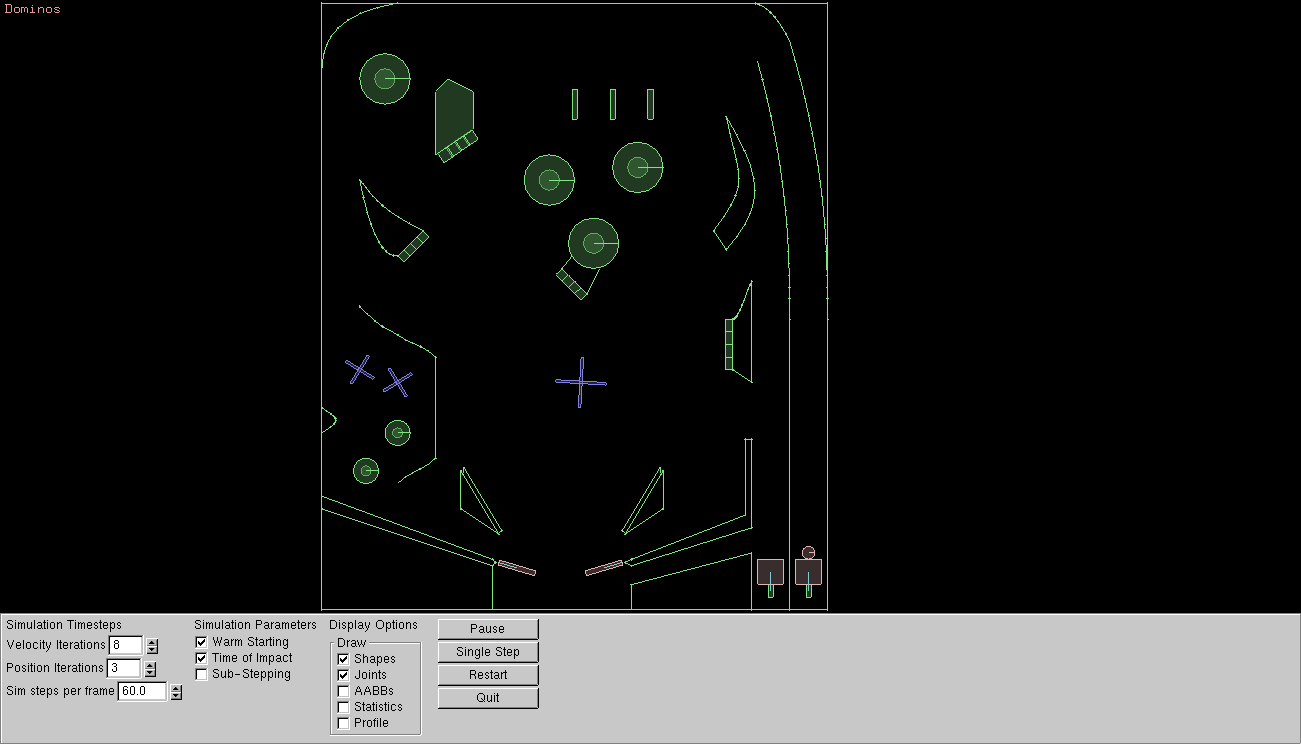
\includegraphics[width=2.65in,natwidth=610,natheight=642]{userInterface.png}
 	  \end{figure}
\end{itemize}
}

\subsection{Play}
\frame{\frametitle{Playing the Game}
\begin{itemize}
\item<1->To launch the ball we need to use the button W.
\item<2->We've implemented the launcher mechanism using prismatic joint.
\item<3->We can control the flippers by using A , D.
\item<4->The flippers are made using a revolute joint with an invisible body.
\item<5->The second launcher can be controlled using 8.
\item<6->The flipper wheel can be rotated using 4 , 6 in the desired direction.
\end{itemize}
}

\frame{\frametitle{Playing the Game}
Here are some of the images in between the game.
\begin{minipage}[t]{0.25\textwidth}
        \vspace{0pt}
        \centering
        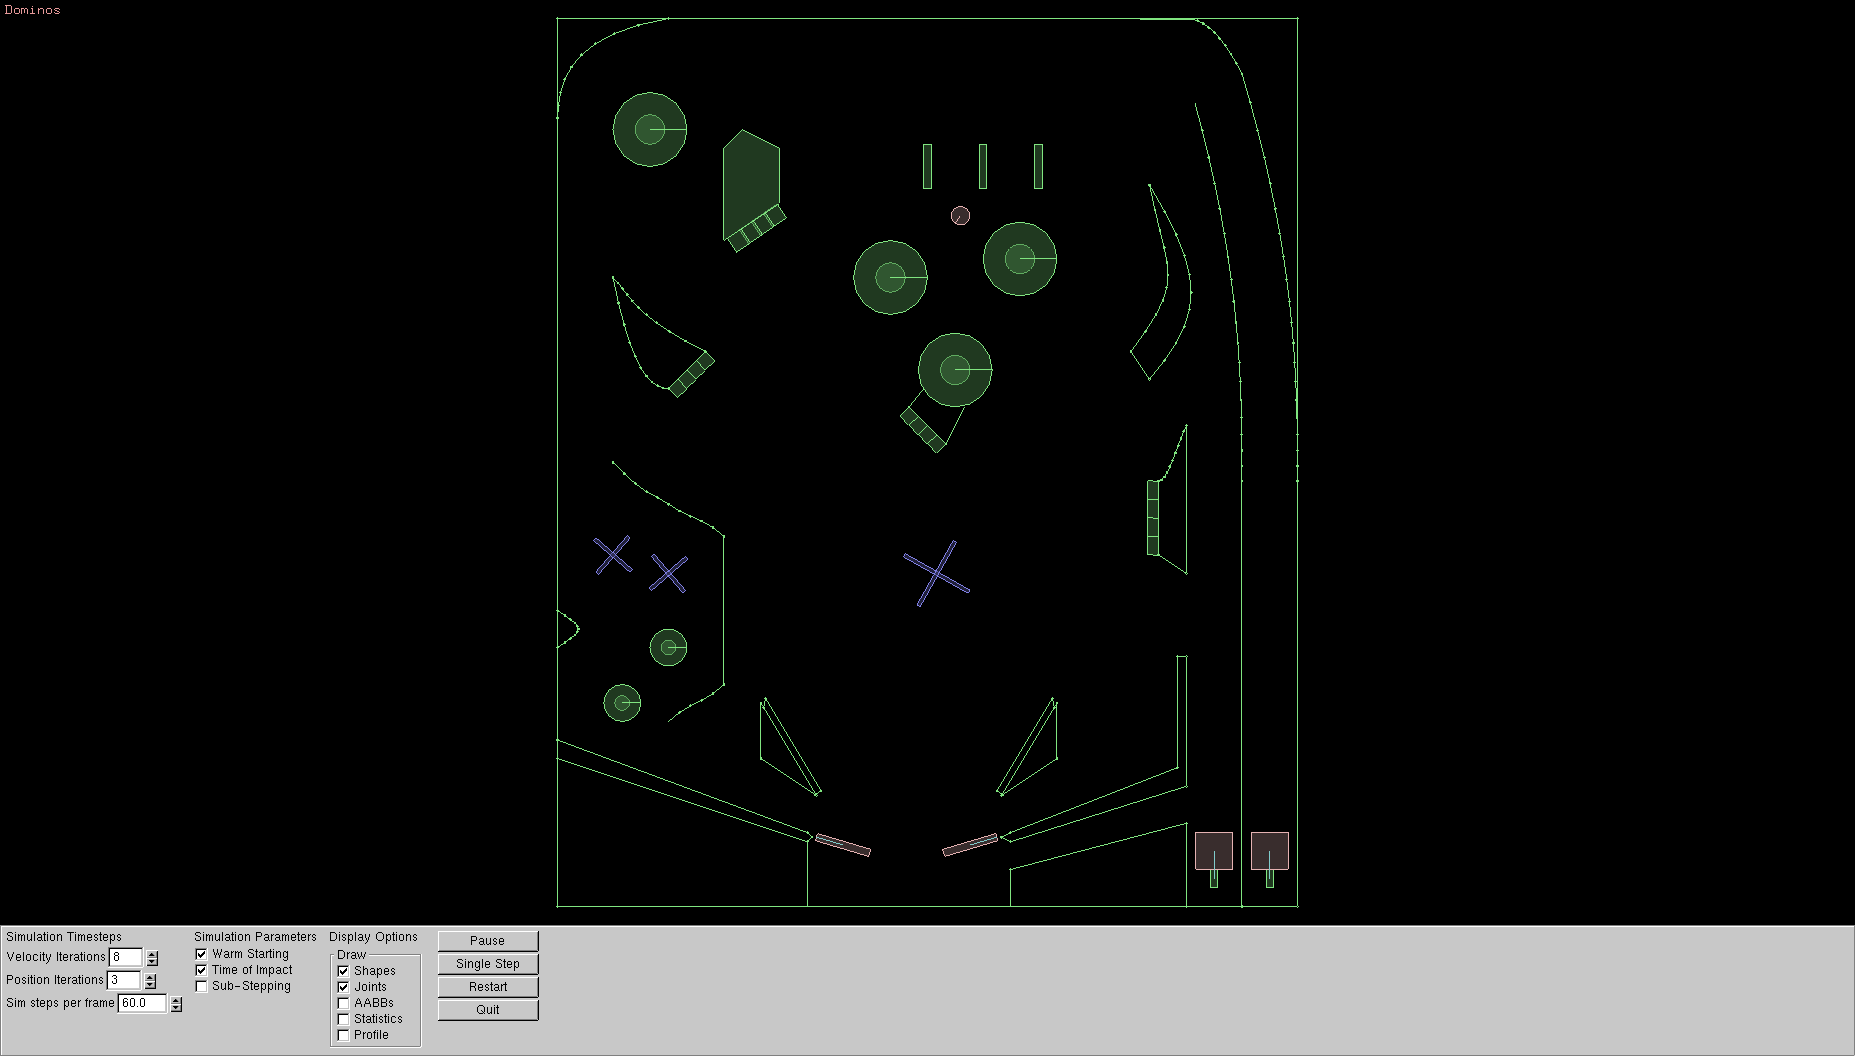
\includegraphics[width=1.3\linewidth,natwidth=610,natheight=642]{play1.png} 
        \label{fig:game}
\end{minipage}
\hspace{1cm}
\begin{minipage}[t]{0.25\textwidth}
        \vspace{0pt}
        \centering
        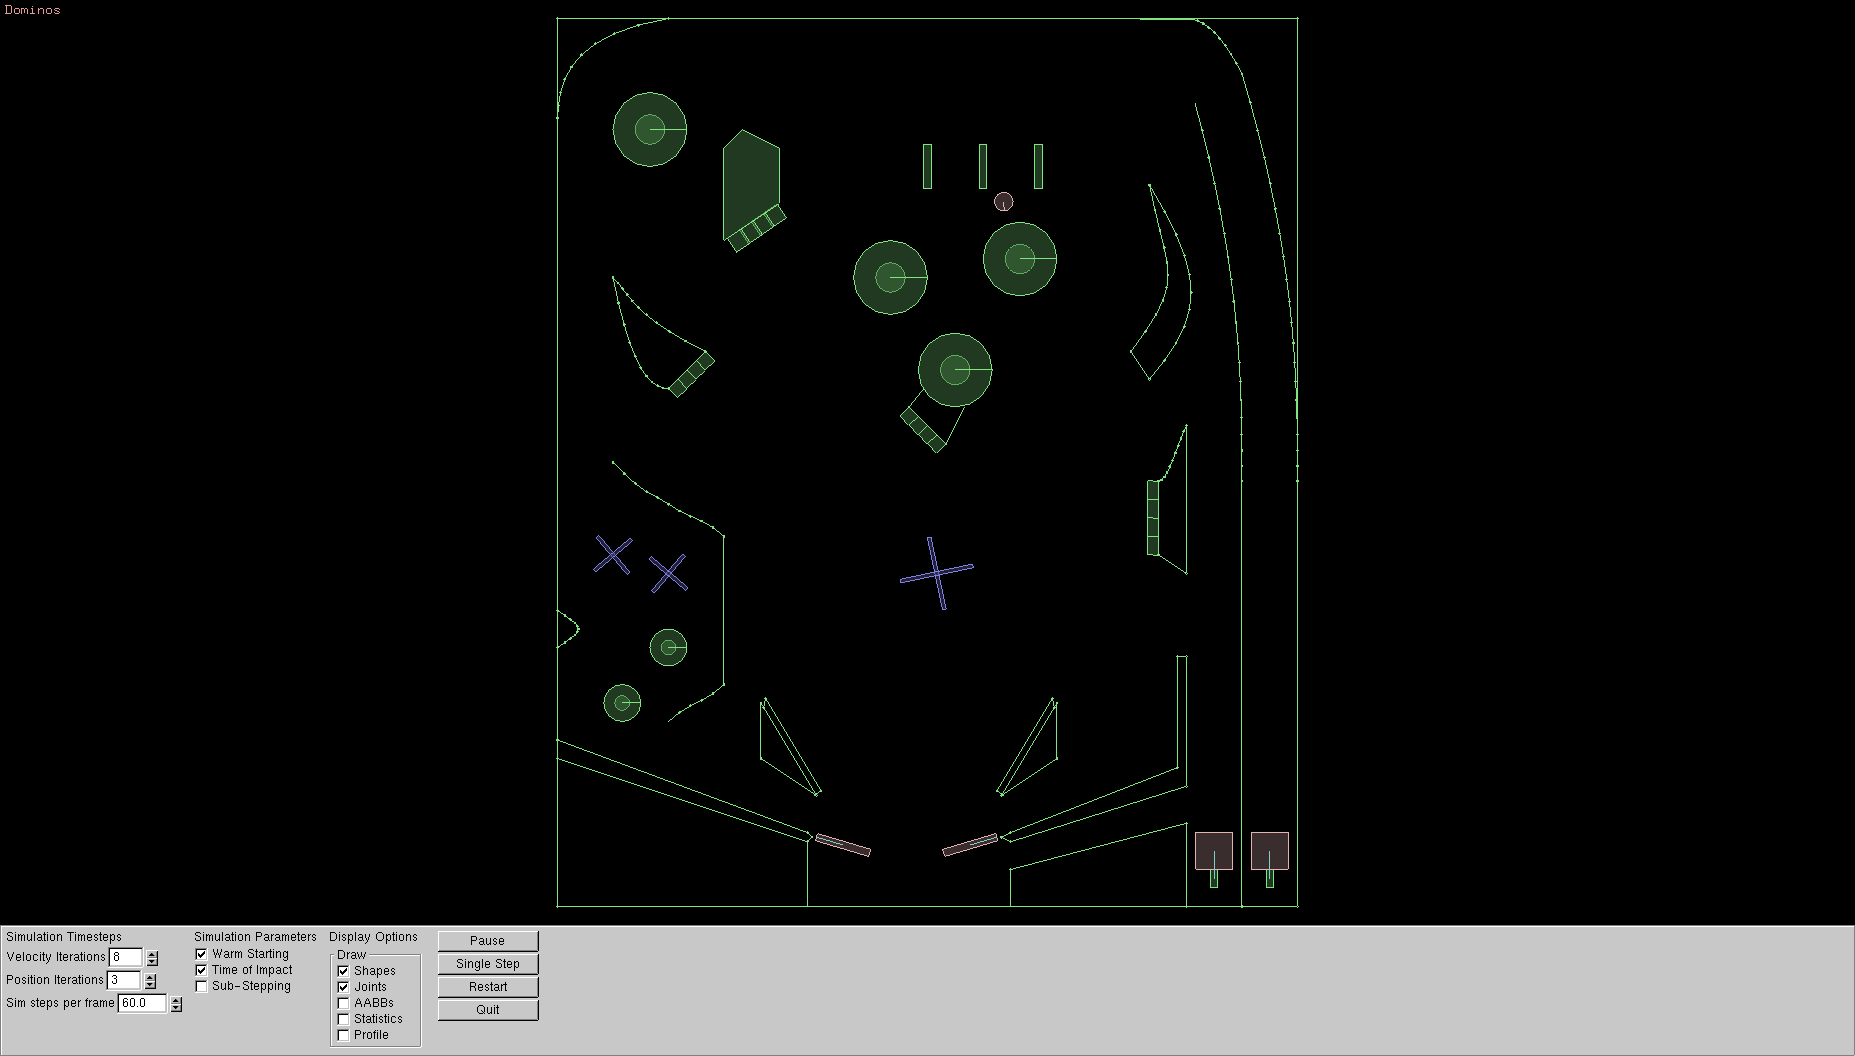
\includegraphics[width=1.3\linewidth,natwidth=610,natheight=642]{play2.png}
        \label{fig:game}
\end{minipage}
\hspace{1cm}
\begin{minipage}[t]{0.25\textwidth}
        \vspace{0pt}
        \centering
        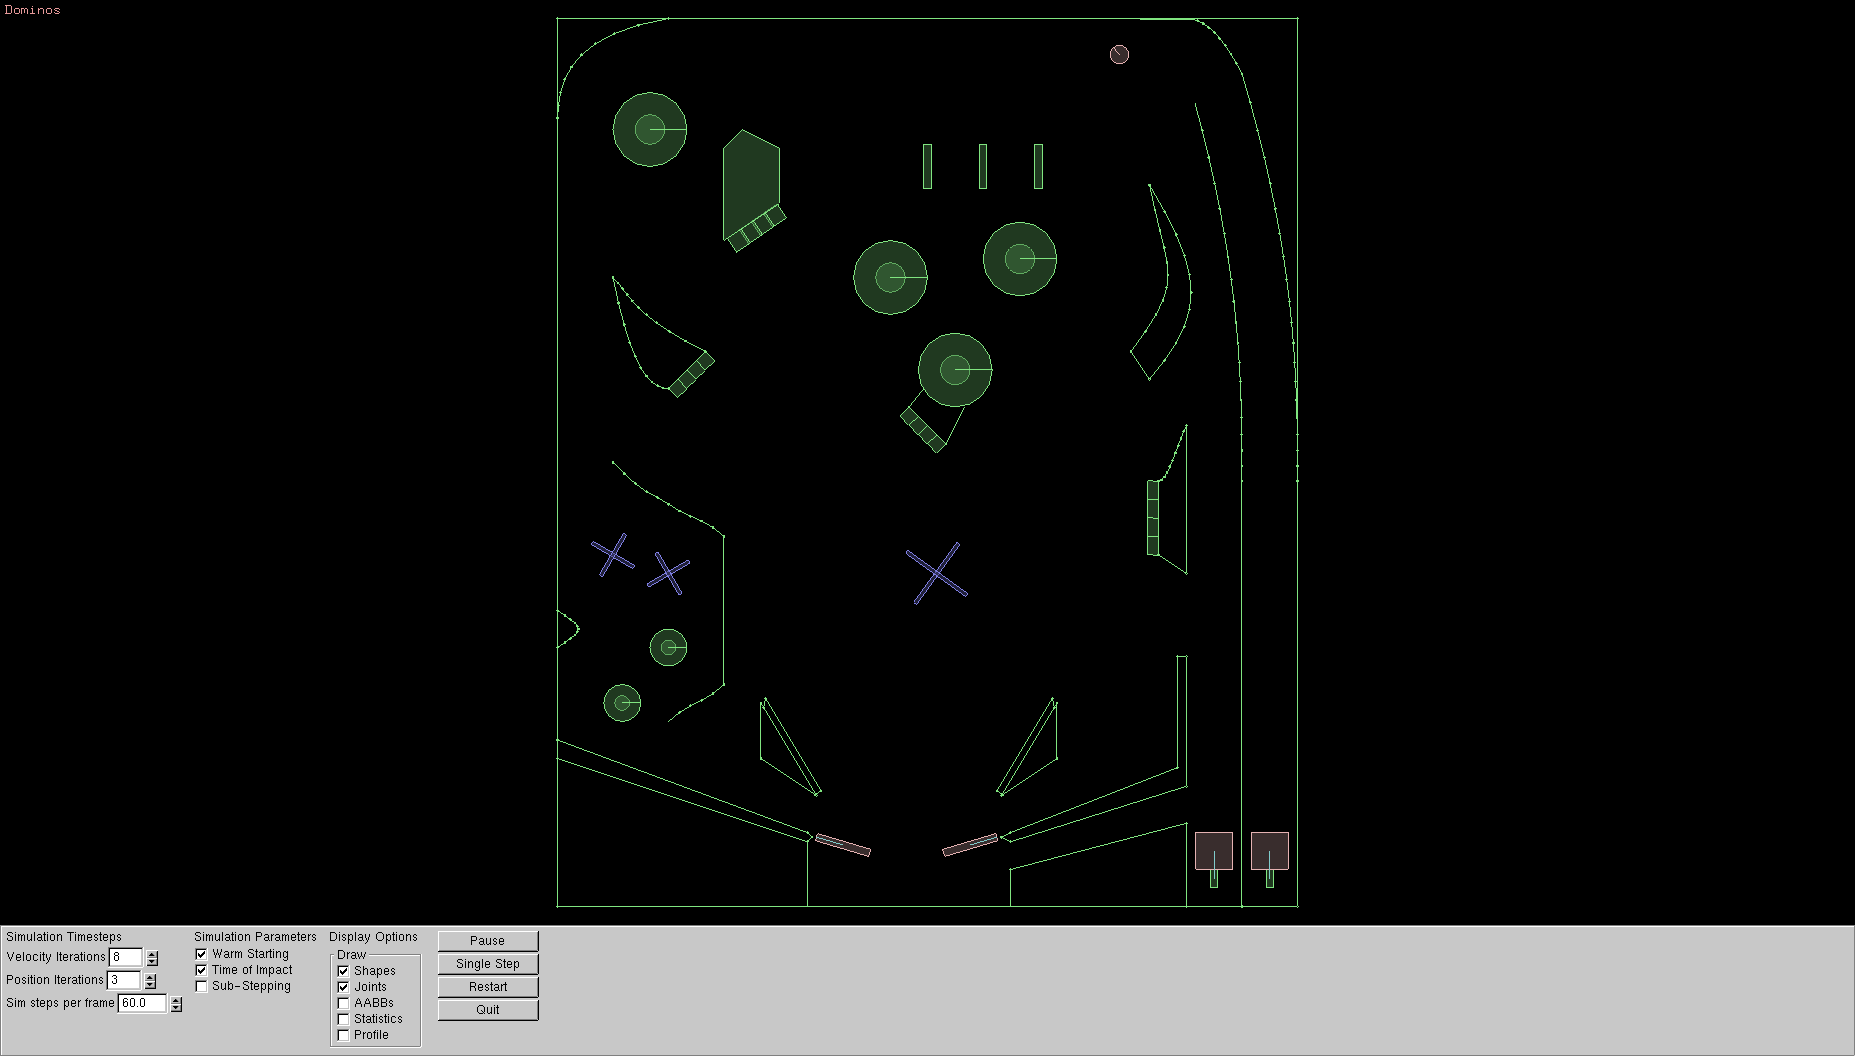
\includegraphics[width=1.3\linewidth,natwidth=610,natheight=642]{play3.png}
        \label{fig:game}
\end{minipage}
}

\subsection{End}
\frame{\frametitle{Playing the Game}
\begin{itemize}
\item<1->The game ends when the ball falls down the flippers.
	\begin{figure}
	    \centering
	    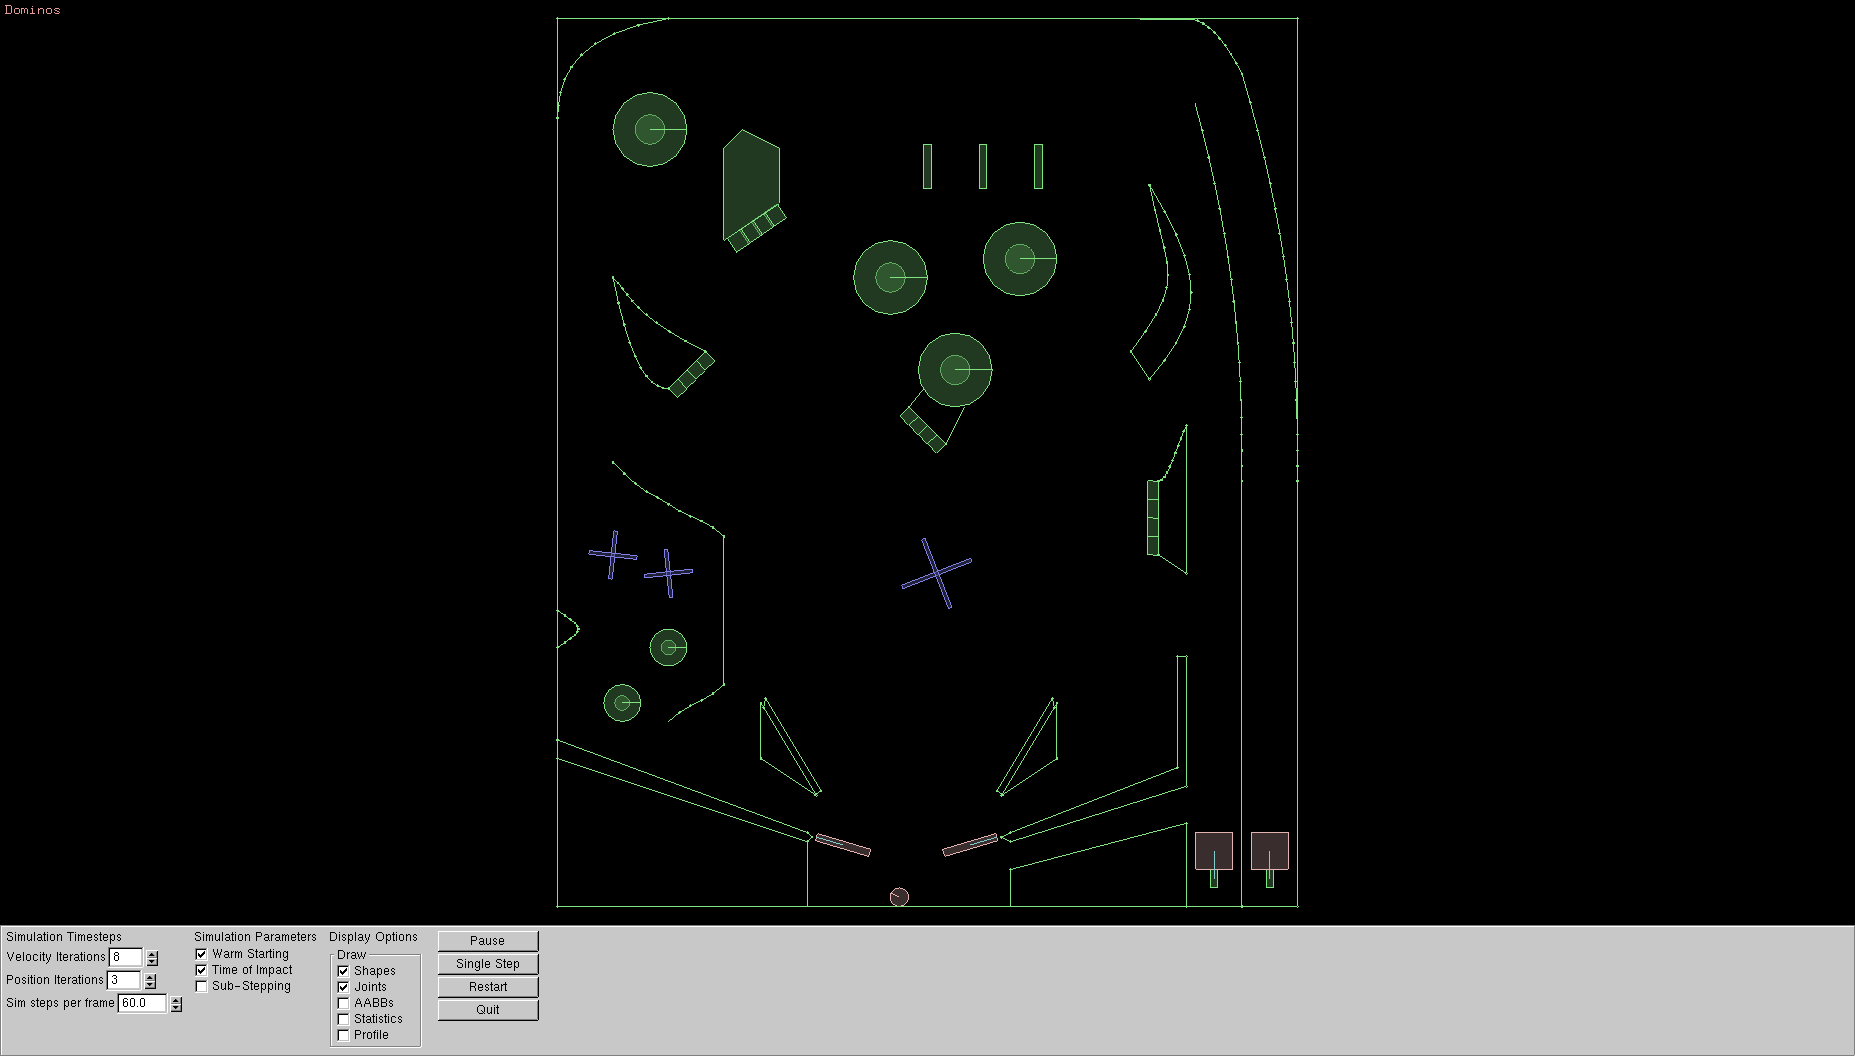
\includegraphics[width=2.65in,natwidth=610,natheight=642]{end.png}
 	  \end{figure}
\end{itemize}
}

\section{Conclusion} 
\frame{\frametitle{Conclusion}
Thanks for going through our presentation.\\
We hope this presentation has served the purpose to get you more enthusiastic about checking out our game.\\
Thank You!!
}

\end{document}